% Chapter 12 -- Verilog II: testbenches and the classic bugs
\chapter{Verilog II: testbenches and the classic bugs}\label{ch:verilog2}

Chapter~11 taught the language. This chapter teaches the discipline
around it, because most of your Verilog hours will not be spent writing
modules --- they will be spent finding out \emph{why the module you
already wrote is lying to you}. A testbench is where design meets its
mirror: a throwaway module whose only job is to drive the real one and
grade its answers. We open the bench like a machine --- clock,
stimulus, check, report --- then walk the five classic bugs one by
one, each caught on tape by a real run. By the end you can write a
bench that prints a verdict, and read any of the classic failures
straight off the monitor rows.

\section{The anatomy of a clocked testbench}\label{sec:anatomy}

\index{testbench}\index{DUT|see{design under test}} A clocked
testbench has four organs (Figure~\ref{fig:tbanatomy}). Everything
inside is \emph{behavioural} --- full software rules apply, because
the bench is never synthesized:

\begin{description}
\item[Clock generator.] A free-running
\texttt{always \#5 clk=\textasciitilde clk;} produces the heartbeat
every sequential design needs. The bench owns time; the DUT merely
reacts to it.
\item[Stimulus.] An \texttt{initial} block pokes inputs with
\texttt{\#} delays. In a program this is a script; in the bench it is
the entire reason to exist. Drive inputs on the \emph{quiet} part of
the cycle (\S\ref{sec:race} shows why).
\item[Check.] Something compares what came out against what should
have: a \texttt{\$monitor} you read, a \texttt{task} that counts
errors, or a golden model running alongside
(\S\ref{sec:selfcheck}).
\item[Report.] Two counters --- \texttt{n} checks, \texttt{errors}
--- and one verdict line, then \texttt{\$finish}. A run that ends in
silence is a run nobody checked.
\end{description}

\begin{figure}[htbp]
\centering
% fig_tbanatomy.tex -- the four organs of a clocked testbench
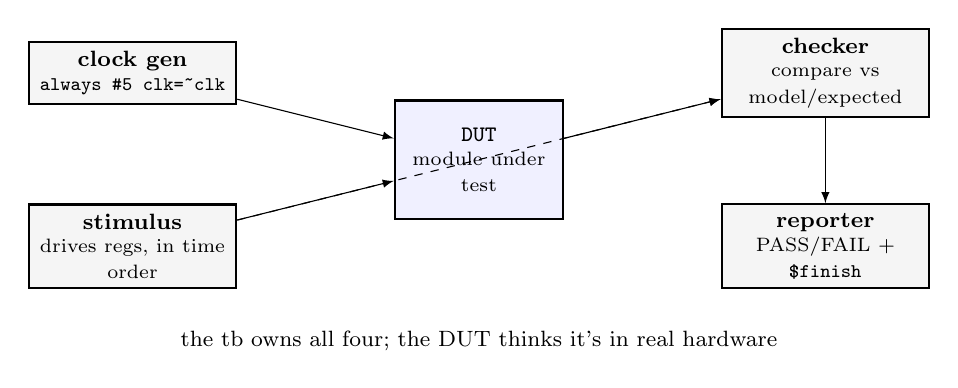
\begin{tikzpicture}[font=\footnotesize, >=latex]
  \node[draw, thick, fill=blue!6, minimum width=2.1cm, minimum height=1.5cm]
    (dut) at (0,0) {\parbox{1.9cm}{\centering \texttt{DUT}\\[-1pt]{\scriptsize module under test}}};
  \node[draw, thick, fill=gray!8, minimum width=2.6cm] (clk) at (-4.4,1.1)
    {\parbox{2.4cm}{\centering \textbf{clock gen}\\[-1pt]{\scriptsize\texttt{always \#5 clk=\textasciitilde clk}}}};
  \node[draw, thick, fill=gray!8, minimum width=2.6cm] (stim) at (-4.4,-1.1)
    {\parbox{2.4cm}{\centering \textbf{stimulus}\\[-1pt]{\scriptsize drives regs, in time order}}};
  \node[draw, thick, fill=gray!8, minimum width=2.6cm] (chk) at (4.4,1.1)
    {\parbox{2.4cm}{\centering \textbf{checker}\\[-1pt]{\scriptsize compare vs model/expected}}};
  \node[draw, thick, fill=gray!8, minimum width=2.6cm] (rpt) at (4.4,-1.1)
    {\parbox{2.4cm}{\centering \textbf{reporter}\\[-1pt]{\scriptsize PASS/FAIL + \texttt{\$finish}}}};
  \draw[->] (clk) -- (dut); \draw[->] (stim) -- (dut);
  \draw[->] (dut) -- (chk); \draw[->] (chk) -- (rpt);
  \draw[dashed, ->] (stim) -- (chk);
  \node[align=center] at (0,-2.3)
    {the tb owns all four; the DUT thinks it's in real hardware};
\end{tikzpicture}

\caption{The four organs of a clocked bench. Notice the ownership:
everything on the left drives the DUT; everything on the right grades
it. The dashed line is the lazy path --- reading stimulus into checks
works, but a golden model (\S\ref{sec:selfcheck}) does it honestly.}
\label{fig:tbanatomy}
\end{figure}

\begin{rulebox}[The bench owns time]
Everything the DUT sees --- edges, input changes, the end of the
world --- is scheduled by the bench. If a transition happens without
your say-so, something in the bench is driving it; find it. There are
no spontaneous events in simulation.
\end{rulebox}

\begin{exercise}[easy]
Label the four organs in \texttt{code/ch12\_xcounter\_tb.v}. Which
line is the clock, which is stimulus, which is check, which is
report?
\end{exercise}

\section{\$display, \$finish and the severity family}
\label{sec:severity}

\index{\$display@\texttt{\$display}}\index{\$monitor@\texttt{\$monitor}}%
\index{\$finish@\texttt{\$finish}} Three printing verbs cover most
runs. \texttt{\$display(fmt,...)} prints once, when its line executes
--- put it inside a clocked block to sample settled values.
\texttt{\$monitor(fmt,...)} prints \emph{every time a printed signal
changes} --- one line arms it for the whole run; it is the text-mode
waveform. \texttt{\$finish} ends the world; every bench must reach it
or the sim spins forever.

SystemVerilog (and Icarus 13) also know the severity tasks
\texttt{\$info}, \texttt{\$warning}, \texttt{\$error},
\texttt{\$fatal(n,~msg)} --- print at escalating alarm levels;
\texttt{\$fatal} kills the run with an exit code. The bigger
\texttt{\$assert} machinery is SystemVerilog territory we reach for
later; today a five-line \texttt{task} does the same job honestly.

\section{Worked example 1: a bench that reports, not just prints}
\label{sec:we-report}

\textbf{Strategy.} Wrap the verdict in a \texttt{check} task: one
counter for checks, one for errors, a message on every failure, a
final line that states the score. Then plant a check we know fails
and watch the machinery bite.

\textbf{Solution.}
\begin{lstlisting}[caption={\ttfamily code/ch12\_report\_tb.v ---
the check/report pattern in 18 lines. Notice the string argument
width \texttt{[8*24-1:0]}: Icarus truncates narrower task strings.},
label={lst:report}]
`timescale 1ns/1ps
module report_tb;
  integer n = 0, errors = 0, warns = 0;
  task check(input cond, input [8*24-1:0] what);
    if (cond) n = n + 1;
    else begin
      errors = errors + 1;
      $display("%0t ERROR %0s failed", $time, what);
    end
  endtask
  initial begin
    $display("--- tb start ---");
    check(4 == 4,   "add table row");
    check(15 == 15, "terminal count");
    check(0 === 1'bx, "planted x compare");
    if (errors > 4) $fatal(1, "too many errors, aborting");
    $display("--- tb done: %0d checks, %0d errors ---", n, errors);
    $finish;
  end
endmodule
\end{lstlisting}

\begin{lstlisting}[caption={Real run. Notice the planted line: one
ERROR, named, with the sim time; the verdict prints the honest score
2/3.},abovecaptionskip=0pt,label={lst:reportout}]
--- tb start ---
0 ERROR planted x compare failed
--- tb done: 2 checks, 1 errors ---
\end{lstlisting}

The planted failure is a lesson in itself: \texttt{===} is the
\emph{case equality}\index{case equality} operator --- it compares
\texttt{x} and \texttt{z} literally. \texttt{0 === 1'bx} is false, so
it fails; \texttt{0 == 1'bx} would \emph{also} be false but for the
wrong reason (\texttt{==} against \texttt{x} yields \texttt{x}, which
an \texttt{if} reads as false). When you mean ``must equal this exact
pattern'', write \texttt{===}; when you mean ``must differ, even
against unknowns'', write \texttt{!==}\index{case inequality}.

\section{The classic bugs}\label{sec:bugs}

Five bugs account for nearly all first-month Verilog pain
(Figure~\ref{fig:bugcat}). Two you met in ch11 --- the inferred latch
and blocking-in-sequential --- return here as named suspects; three
are new: un-reset \texttt{x} forever, the missing \texttt{default},
and the bench fighting the DUT. Every one is demonstrated below with
a run you can repeat.

\begin{figure}[htbp]
\centering
% fig_bugcat.tex -- the bug catalogue card
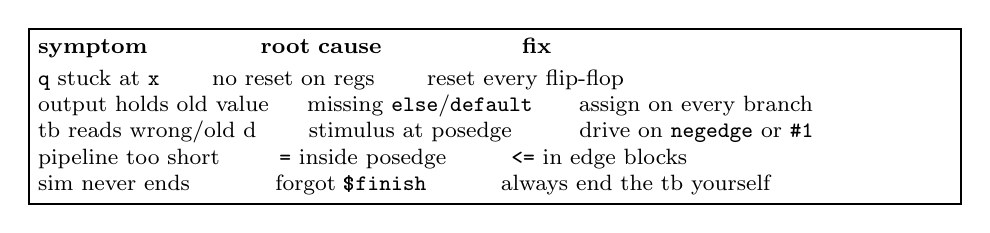
\begin{tikzpicture}[font=\footnotesize]
  \node[draw, thick, text width=11.6cm, align=left] at (0,0) {%
  \textbf{symptom \hspace{3.6em} root cause \hspace{4.6em} fix}\\[2pt]
  \texttt{q} stuck at \texttt{x}\hspace{1.9em} no reset on regs\hspace{1.9em}
    reset every flip-flop\\
  output holds old value\hspace{1.3em} missing \texttt{else}/\texttt{default}
    \hspace{1.3em} assign on every branch\\
  tb reads wrong/old d\hspace{1.9em} stimulus at posedge
    \hspace{2.2em} drive on \texttt{negedge} or \texttt{\#1}\\
  pipeline too short\hspace{2.2em} \texttt{=} inside posedge
    \hspace{2.1em} \texttt{<=} in edge blocks\\
  sim never ends\hspace{3.3em} forgot \texttt{\$finish}
    \hspace{2.5em} always end the tb yourself};
\end{tikzpicture}

\caption{The classic-bug catalogue. Notice that every symptom is
silent --- none of these produce an error message; the bench or your
eyes catch them, which is why this chapter exists.}
\label{fig:bugcat}
\end{figure}

\section{Worked example 2: the x that never leaves}
\label{sec:we-xprop}

\textbf{Strategy.} Registers start life unknown. Simulate the same
counter with and without a reset; watch one count and one rot.

\textbf{Solution.}
\begin{lstlisting}[caption={\ttfamily code/ch12\_xcounter.v --- the
only difference is \texttt{rst}.},label={lst:xcounter}]
module cnt_norst(clk, q);
  input clk; output reg [3:0] q;
  always @(posedge clk) q <= q + 1'b1;   // q starts x -> stays x
endmodule
module cnt_rst(clk, rst, q);
  input clk, rst; output reg [3:0] q;
  always @(posedge clk)
    if (rst) q <= 4'd0; else q <= q + 1'b1;
endmodule
\end{lstlisting}

\begin{lstlisting}[caption={Real run of \ttfamily
ch12\_xcounter\_tb.v. Notice: \texttt{x + 1 = x} forever --- arithmetic
on unknowns produces unknowns --- while the reset twin wakes at t=5
and counts.},abovecaptionskip=0pt,label={lst:xcounterout}]
t= 0 | no-rst q=xxxx | with-rst q=xxxx
t= 5 | no-rst q=xxxx | with-rst q=0000
t=25 | no-rst q=xxxx | with-rst q=0001
t=35 | no-rst q=xxxx | with-rst q=0010
t=45 | no-rst q=xxxx | with-rst q=0011
t=55 | no-rst q=xxxx | with-rst q=0100
\end{lstlisting}

\begin{figure}[htbp]
\centering
% fig_xprop.tex -- x propagation: real sim rows of the no-rst counter
\begin{tikzpicture}[font=\footnotesize]
\begin{axis}[width=12cm, height=5.2cm, xlabel={time (ns)},
  xmin=0, xmax=60, ymin=-0.3, ymax=2.4,
  ytick={0.4,1.6}, yticklabels={no-rst q, with-rst q},
  y tick label style={font=\ttfamily\footnotesize},
  x tick label style={font=\footnotesize}, grid=both, grid style={gray!20}]
\addplot[const plot, very thick, red] table[x=t, y expr=0.4+\thisrow{qx}*0.8] {figures/ch12/ch12_xcounter.dat};
\addplot[const plot, very thick, blue] table[x=t, y expr=1.6+\thisrow{qr}*0.8] {figures/ch12/ch12_xcounter.dat};
\node[anchor=west, red] at (axis cs:33,0.75) {x+1 = x forever};
\node[anchor=west, blue] at (axis cs:40,2.25) {reset saved it};
\end{axis}
\end{tikzpicture}

\caption{Real monitor rows from \texttt{ch12\_xcounter.out}, drawn as
a wave pane. Notice the dead lane: \texttt{no-rst q} never leaves
\texttt{x} (mapped mid-band here); the reset twin counts normally.}
\label{fig:xprop}
\end{figure}

\index{x propagation@\texttt{x} propagation}\index{unknown value|see{\texttt{x} propagation}}
This is \emph{x-propagation}: unknown in, unknown out. The sim is
telling you the truth --- real silicon powers up in \emph{a} state,
you just do not know which, and \texttt{x} is the honest label for
``could be anything''. Two habits follow. First, \emph{every
sequential register gets a reset path} (or a documented reason it
needs none). Second, when a waveform shows \texttt{x}, read it as a
question, not a value: ``who was supposed to initialize this?''

\begin{exercise}[medium]
In \texttt{ch12\_xcounter\_tb.v}, drop the reset release
(\texttt{\#25 rst=0;}) and predict both columns before you re-run.
Then re-run.
\end{exercise}

\section{Worked example 3: the case that forgot a branch}
\label{sec:we-caselatch}

\textbf{Strategy.} The inferred latch from ch11 had an \texttt{if}
missing its \texttt{else}. The same bug hides inside \texttt{case}
when an input combination is simply absent --- no warning, clean
synthesis, wrong hardware. Give a 4-way ALU an
\texttt{op=11} gap and watch it hold the previous answer.

\textbf{Solution.}
\begin{lstlisting}[caption={\ttfamily code/ch12\_caselatch.v ---
identical except the \texttt{default}.},label={lst:caselatch}]
module alu4(op, a, b, y);                // WRONG: 2'b11 missing
  input [1:0] op; input [3:0] a, b; output reg [3:0] y;
  always @(*) case (op)
    2'b00: y = a + b;
    2'b01: y = a - b;
    2'b10: y = a & b;
    // 2'b11 silently missing -> y holds old value
  endcase
endmodule
module alu4safe(op, a, b, y);
  input [1:0] op; input [3:0] a, b; output reg [3:0] y;
  always @(*) case (op)
    2'b00: y = a + b;
    2'b01: y = a - b;
    2'b10: y = a & b;
    default: y = 4'b0000;    // explicit, no latch
  endcase
endmodule
\end{lstlisting}

\begin{lstlisting}[caption={Real run. Notice \texttt{op=11} at t=20:
the latched ALU answers 5 --- a \emph{memory} of the subtraction ---
while the safe one answers 0. The latch is not a bug you see; it is a
bug that sees you.},abovecaptionskip=0pt,label={lst:caselatchout}]
t= 0 op=00 a= 7 b= 2 | latched= 9 safe= 9
t=10 op=01 a= 7 b= 2 | latched= 5 safe= 5
t=20 op=11 a= 7 b= 2 | latched= 5 safe= 0
t=30 op=00 a= 7 b= 2 | latched= 9 safe= 9
\end{lstlisting}

\index{inferred latch}The fix is boring and absolute: in a
combinational block, \emph{every output is assigned on every path}.
Two styles do it --- a \texttt{default} arm, or an unconditional
assignment before the \texttt{case} (\texttt{y = 0; case...}). Both
kill the latch; the second also documents the ``don't care'' value.

\section{The race you cannot see}\label{sec:race}

\index{race condition (simulation)}The strangest classic bug changes
nothing in your hardware and still breaks the sim. Simulation time is
quantised: at a \texttt{posedge}, the DUT samples \texttt{d}
\emph{and} the bench may also be changing \texttt{d} --- in the same
instant. Who wins is a coin flip inside the simulator's event queue.
Your design is fine; your bench is unreliable.

\section{Worked example 4: the same flip-flop, two benches}
\label{sec:we-race}

\textbf{Strategy.} One DFF, two benches. The bad one toggles
\texttt{d} exactly \emph{at} \texttt{posedge clk}; the good one does
it at \texttt{negedge} --- the quiet midpoint where nothing samples.

\textbf{Solution.}
\begin{lstlisting}[caption={\ttfamily code/ch12\_race\_tb.v
(abridged) --- one line differs.},label={lst:race}]
// BAD: stimulus changes in the same instant the clock edges.
module race_bad_tb;
  reg clk=0, d=0; wire q;
  dff2 u(.clk(clk), .d(d), .q(q));
  always #5 clk=~clk;
  always @(posedge clk) d = ~d;          // races the DFF's sample!
  initial $monitor("t=%2d clk=%b d=%b q=%b", $time, clk, d, q);
  initial #40 $finish;
endmodule
// GOOD: drive on the opposite edge (or #1 after) - no ambiguity.
module race_good_tb;
  ...
  always @(negedge clk) d = ~d;          // settled half a cycle early
  ...
endmodule
\end{lstlisting}

\begin{lstlisting}[caption={Real run, \texttt{race\_bad\_tb}. Notice:
\texttt{d} toggles cleanly but \texttt{q} pins at 1 --- the DUT keeps
sampling the \emph{new} \texttt{d}, a stable wrong answer with no
error message anywhere.},abovecaptionskip=0pt,label={lst:racebad}]
t= 5 clk=1 d=1 q=1
t=15 clk=1 d=0 q=1
t=25 clk=1 d=1 q=1
t=35 clk=1 d=0 q=1
\end{lstlisting}

\begin{lstlisting}[caption={Real run, \texttt{race\_good\_tb}. Same
DUT, stimulus moved to \texttt{negedge}: \texttt{q} now follows
\texttt{d} one edge behind, as a flip-flop
must.},abovecaptionskip=0pt,label={lst:racegood}]
t= 5 clk=1 d=0 q=0
t=15 clk=1 d=1 q=1
t=25 clk=1 d=0 q=0
t=35 clk=1 d=1 q=1
\end{lstlisting}

\begin{figure}[htbp]
\centering
% fig_race.tex -- the tb/DUT race cartoon
\begin{tikzpicture}[font=\footnotesize, >=latex]
  \draw[->] (0,0) -- (9.2,0) node[right]{time};
  \foreach \x/\l in {2/posedge, 7/posedge}{
    \draw[dashed, gray] (\x,0) -- (\x,3.0); \node[below] at (\x,0) {\l}; }
  \draw[thick] (0,0.15) -- (2,0.15) -- (2,0.75) -- (7,0.75) -- (7,0.15) -- (9,0.15);
  \node[left] at (0,0.45) {clk};
  \node[left] at (0,1.6) {BAD:};
  \draw[thick, red] (2,1.35) -- (2,1.95) -- (9,1.95);
  \node[right, red, align=left] at (9,1.65) {d changes IN the edge\\ --- who saw old d?};
  \node[left] at (0,2.6) {GOOD:};
  \draw[thick, good] (4.5,2.35) -- (4.5,2.95) -- (9,2.95);
  \node[right, good, align=left] at (9,2.65) {d settles mid-cycle\\ --- posedge unambiguous};
\end{tikzpicture}

\caption{Why the race exists. Notice that the \emph{same instant}
carries two writers: the bench changes \texttt{d} exactly when the
DUT samples it. Moving the write to mid-cycle leaves a clean window
on either side of the edge.}
\label{fig:race}
\end{figure}
\begin{figure}[htbp]
\centering
\begin{tikzpicture}
\begin{axis}[
    width=0.92\linewidth, height=4.4cm,
    axis lines=left,
    xlabel={time $t$}, xlabel style={font=\footnotesize},
    ymin=-0.4, ymax=3.6, ytick=\empty,
    clip=false,
    xmin=0, xmax=42, tick label style={font=\footnotesize},
    title={\footnotesize bad bench: stimulus at \texttt{posedge}},
    title style={font=\footnotesize},
]
\addplot+[const plot, line width=1.1pt, accent, mark=*, mark size=0.7pt]
  table[x=t,y=db] {figures/ch12/ch12_race.dat};
\addplot+[const plot, line width=1.1pt, good, mark=square*, mark size=0.7pt]
  table[x=t,y expr=\thisrow{qb}+2.25] {figures/ch12/ch12_race.dat};
\node[anchor=east, font=\footnotesize] at (axis cs:-1,0.5) {d};
\node[anchor=east, font=\footnotesize] at (axis cs:-1,2.75) {q};
\end{axis}
\end{tikzpicture}\\[2pt]
\begin{tikzpicture}
\begin{axis}[
    width=0.92\linewidth, height=4.4cm,
    axis lines=left,
    xlabel={time $t$}, xlabel style={font=\footnotesize},
    ymin=-0.4, ymax=3.6, ytick=\empty,
    clip=false,
    xmin=0, xmax=42, tick label style={font=\footnotesize},
    title={\footnotesize good bench: stimulus at \texttt{negedge}},
    title style={font=\footnotesize},
]
\addplot+[const plot, line width=1.1pt, accent, mark=*, mark size=0.7pt]
  table[x=t,y=dg] {figures/ch12/ch12_race.dat};
\addplot+[const plot, line width=1.1pt, good, mark=square*, mark size=0.7pt]
  table[x=t,y expr=\thisrow{qg}+2.25] {figures/ch12/ch12_race.dat};
\node[anchor=east, font=\footnotesize] at (axis cs:-1,0.5) {d};
\node[anchor=east, font=\footnotesize] at (axis cs:-1,2.75) {q};
\end{axis}
\end{tikzpicture}
\caption{Same flip-flop, two benches (Listing~\ref{lst:race}). Top: stimulus driven
\textit{at} \texttt{posedge} --- $d$ still toggles but $q$ is stuck at~1, because the
bench and the DUT fight over who changes first. Bottom: stimulus moved to
\texttt{negedge} --- $q$ now samples the settled $d$ and toggles correctly, one edge
behind. Rows are the real \texttt{\$monitor} output, parsed from
\texttt{code/ch12\_race\_*.out}.}
\label{fig:racewave}
\end{figure}


The discipline that deletes this bug forever: \emph{change stimulus
on the clock edge the DUT does not listen to} --- or equivalently,
drive \texttt{d} with \texttt{\#1} after the active edge so it lands
in settled territory. Hardware has setup/hold windows; the sim
punishes you for pretending they are zero.

\begin{exercise}[medium]
Predict: in \texttt{race\_good\_tb}, at t=25 \texttt{q} is sampled
from which value of \texttt{d}, set when? Confirm against
\texttt{code/ch12\_race\_good.out}.
\end{exercise}

\section{Blocking in sequential, one line}\label{sec:blockingrecap}

Chapter~11's pipeline demo is the proof on tape
(\S\ref{sec:we-pipe}): \texttt{=} inside a \texttt{posedge} block lets
a later line read the \emph{new} value, collapsing a two-flop
pipeline into one. It earns its row in the classic-bugs table and one
line here: \textbf{edge blocks get \texttt{<=}, always}. The bug is
silent --- no x, no latch report --- which is exactly why it is in
the top five.

\section{Self-checking patterns}\label{sec:selfcheck}

\index{self-checking testbench}Benches grade on a sliding scale of
effort versus catch-rate:

\begin{description}
\item[Eyeball.] \texttt{\$monitor} rows or a wave pane you read
yourself. Fine for bring-up; useless the day you change one line and
do not re-read the wave.
\item[Directed checks.] Expected values in the bench, one
\texttt{check} per row --- ch11's counter. Catches exactly what you
thought to test.
\item[Golden model.] A second, trusted implementation --- usually
simpler, often not synthesizable --- running next to the DUT,
compared on every event. Catches what you did \emph{not} think to
test, which is where bugs live.
\end{description}

\section{Worked example 5: the golden model catches a 1-bit bug}
\label{sec:we-golden}

\textbf{Strategy.} Plant a bug small enough to eyeball past: a shift
register whose update carries a stray \texttt{\^{}}. A golden copy
--- one line of spec-level Verilog --- runs in the same bench and
compares every edge.

\textbf{Solution.}
\begin{lstlisting}[caption={\ttfamily code/ch12\_shift.v --- spot the
bug; the model does not care that you can't.},label={lst:shift}]
module shift8(clk, en, sin, q);
  input clk, en, sin; output reg [7:0] q;
  always @(posedge clk)
    if (en) q <= {q[6:0], sin} ^ 8'b1;   // subtle bug: extra XOR bit0
endmodule
\end{lstlisting}

\begin{lstlisting}[caption={\ttfamily code/ch12\_golden\_tb.v
(abridged) --- the spec runs inside the bench. Notice
\texttt{\#1}: read the DUT \emph{after} the edge settles, the
\texttt{negedge}-style discipline of \S\ref{sec:race}.},
label={lst:golden}]
module golden_tb;
  reg clk=0, en=0, sin=0;
  wire [7:0] q;
  shift8 u(.clk(clk), .en(en), .sin(sin), .q(q));
  reg [7:0] model = 0;                    // the golden copy
  integer errors = 0;
  always #5 clk=~clk;
  always @(posedge clk) #1 begin         // run the model alongside
    if (en) model = {model[6:0], sin};   // what shift SHOULD do
    if (q !== model) begin
      errors = errors + 1;
      $display("MISMATCH t=%0d q=%b model=%b", $time, q, model);
    end
  end
  ...
\end{lstlisting}

\begin{lstlisting}[caption={Real run. Notice two things: the early
rows are un-reset \texttt{x} surfacing (\S\ref{sec:we-xprop} ---
\texttt{!==} treats them as mismatches, honestly), and t=46 shows the
planted bug itself --- bit~0 flipped, exactly the XOR's
signature.},abovecaptionskip=0pt,label={lst:goldenout}]
MISMATCH t=6 q=xxxxxxx0 model=00000001
MISMATCH t=16 q=xxxxxx01 model=00000010
MISMATCH t=26 q=xxxxx011 model=00000100
MISMATCH t=36 q=xxxx0111 model=00001000
MISMATCH t=46 q=xxxx0111 model=00001000
FAIL: 5 mismatches
\end{lstlisting}

\begin{figure}[htbp]
\centering
% fig_golden.tex -- golden-model testbench architecture
\begin{tikzpicture}[font=\footnotesize, >=latex]
  \node[draw, thick, fill=gray!8] (stim) at (0,1.6) {stimulus};
  \node[draw, thick, fill=blue!8, minimum width=2.5cm] (dut) at (0,0.5)
    {\texttt{DUT} (real design)};
  \node[draw, thick, fill=amber!15, minimum width=2.5cm] (mod) at (0,-0.9)
    {\texttt{model} (tb's clean copy)};
  \node[draw, thick, fill=red!8] (cmp) at (3.8,-0.2) {\texttt{!==} compare};
  \node[draw, thick] (ver) at (7,-0.2) {PASS / FAIL};
  \draw[->] (stim) -- (dut); \draw[->] (stim) -- (mod);
  \draw[->] (dut.east) -- (cmp); \draw[->] (mod.east) -- (cmp);
  \draw[->] (cmp) -- (ver);
  \node[align=center] at (3.9,-1.9) {the tb re-implements the spec;\\
   every mismatch is a bug, in either copy};
\end{tikzpicture}

\caption{Golden-model architecture. Notice the compare is
\texttt{!==}, not \texttt{!=} --- the point is that \texttt{x} counts
as a mismatch, so un-reset state fails loudly instead of passing
silently.}
\label{fig:golden}
\end{figure}

Two details make the pattern honest. The compare uses
\texttt{!==}\index{case inequality} --- \texttt{!=} against an
\texttt{x} yields \texttt{x} and silently skips the check. And the
model is written at the \emph{spec} level --- what shift should do,
not how the DUT does it --- or you have built two copies of the same
bug.

\begin{exercise}[hard]
Write a golden-model bench for ch09's \texttt{adder4}: the model is
one line (\texttt{wire [4:0] sum = a + b;}), checked every
\texttt{\#1} after inputs change across all 256 input pairs.
\end{exercise}

\section{Reading the wave}\label{sec:waveread}

\index{waveform}Every figure in this chapter was drawn from real
simulator rows --- \texttt{\$monitor} output, or the VCD file
\texttt{\$dumpvars} writes. Reading them back is the skill. Four
habits:

\begin{enumerate}
\item \textbf{Sample on the right instant.} At a \texttt{posedge},
everything the DUT sees is the value \emph{just before} the edge.
A \texttt{\$display} inside the edge block reads pre-update values;
add \texttt{\#1} (or sample at \texttt{negedge}) to read settled
ones --- \S\ref{sec:we-golden} uses this.
\item \textbf{Read x and z first.} \texttt{x} asks ``who initializes
this?''; \texttt{z} asks ``who drives this?''. Both are questions,
not values --- \S\ref{sec:we-xprop}.
\item \textbf{Chase the first wrong edge, not the last.} A bad
\texttt{q} at t=46 was born at t=6. Walk left until the first
disagreement between bench and DUT.
\item \textbf{Trust the bench only after it has lied to you once.}
Run \texttt{-DSABOTAGE}-style checks: plant a wrong expectation and
confirm the machinery reports it (ch11's counter; WE1 here).
\end{enumerate}

\begin{checkpoint}
You can write a clocked testbench with all four organs, wrap checks
in a counting \texttt{task}, name the five classic bugs with one
symptom and one fix each, drive stimulus on the quiet edge, and read
\texttt{x}/\texttt{z} rows as questions about drivers and resets.
\end{checkpoint}

\section{Summary}\label{sec:sum12}

\begin{center}
\begin{tabularx}{\linewidth}{@{}lX@{}}
\toprule
\textbf{Thing} & \textbf{The rule of thumb}\\
\midrule
clocked bench & clock gen + stimulus + check + report; the bench owns time\\
\texttt{\$display}/\texttt{\$monitor} & print-once vs print-on-change; use clocked display to sample settled values\\
\texttt{\$finish}/\texttt{\$fatal} & every bench must terminate; \texttt{\$fatal} for stop-the-line errors\\
\texttt{===}/\texttt{!==} & compare \texttt{x} literally; \texttt{==} hides unknowns\\
inferred latch & every branch assigns every output, or \texttt{default}\\
un-reset \texttt{x} & arithmetic on \texttt{x} gives \texttt{x} forever; reset every register\\
\texttt{=} in edge blocks & pipelines collapse; \texttt{<=} always\\
tb/DUT race & drive stimulus on the idle edge (or \texttt{\#1} later)\\
golden model & spec-level twin + \texttt{!==} every edge\\
\bottomrule
\end{tabularx}
\end{center}

\section{Common mistakes}\label{sec:cm12}

\begin{tripwire}[A counter without a reset]
\texttt{x + 1 = x}, forever --- the sim's most common silent killer.
Give every register a reset path; if one truly needs none, write the
reason in a comment (\S\ref{sec:we-xprop}).
\end{tripwire}
\begin{tripwire}[A \texttt{case} that trusts the inputs]
``\texttt{op} can only be 00--10'' is a promise the hardware cannot
hear. The missing arm is an inferred latch
(\S\ref{sec:we-caselatch}); \texttt{default} costs one line.
\end{tripwire}
\begin{tripwire}[Stimulus at the sampling edge]
Driving \texttt{d} at \texttt{posedge} makes bench and DUT race ---
the output can be stable \emph{and} wrong, with no error message
(\S\ref{sec:we-race}). Drive on the idle edge or \texttt{\#1} later.
\end{tripwire}
\begin{tripwire}[Comparing with \texttt{!=} when \texttt{x} may lurk]
\texttt{q != model} evaluates to \texttt{x} against unknowns and an
\texttt{if} reads that as skip. Self-checkers use
\texttt{!==}/\texttt{===} so \texttt{x} counts as a mismatch
(\S\ref{sec:we-golden}).
\end{tripwire}
\begin{tripwire}[A verdict you never verified]
If your checker has never printed FAIL, you do not know it can.
Plant a wrong expectation once (the \texttt{-DSABOTAGE} habit) and
watch it fire.
\end{tripwire}
\begin{tripwire}[Reading the wave after the edge]
A \texttt{\$display} inside \texttt{@(posedge clk)} sees pre-edge
values --- correct-looking, one cycle stale. \texttt{\#1} after the
edge is where settled truth lives (\S\ref{sec:waveread}).
\end{tripwire}

\begin{exercise}[easy]
\texttt{always @(*) case (s) 1'b0: y = a; endcase} --- what does
\texttt{y} do when \texttt{s=1}? Name the bug and the one-line fix.
\end{exercise}
\begin{exercise}[easy]
Order these for a clean run: \texttt{\$finish}, verdict
\texttt{\$display}, \texttt{\$dumpvars}, stimulus \texttt{initial},
clock \texttt{always}. Which may interleave freely?
\end{exercise}
\begin{exercise}[medium]
A tb drives \texttt{d <= \textasciitilde d} on \texttt{posedge clk}.
Race or fine? Defend in one sentence.
\end{exercise}
\begin{exercise}[medium]
\texttt{check(q === 4'b1010, "pattern")} fails though the wave shows
\texttt{q=1010}. What single character probably differs? (Hint:
upper/lower bits may be \texttt{z}.)
\end{exercise}
\begin{exercise}[medium]
\texttt{\$monitor} prints nothing all run. Name two independent
causes you would check first.
\end{exercise}
\begin{exercise}[medium]
\texttt{model} starts \texttt{= 0}, the DUT starts at \texttt{x}. Is
the t=6 MISMATCH in \S\ref{sec:we-golden} a model bug, a DUT bug, or
a bench-design issue? What two-line change removes it?
\end{exercise}
\begin{exercise}[medium]
You add \texttt{default:;} (empty) to \texttt{alu4}. Latch or no
latch? Run the experiment and say why.
\end{exercise}
\begin{exercise}[medium]
Your FSM bench applies the next input 0\,ns after each
\texttt{posedge}. Which classic bug have you re-created, and what is
the fix?
\end{exercise}
\begin{exercise}[medium]
A shift register is reset \emph{inside} the same
\texttt{@(posedge clk)} block as the shift using \texttt{=}. Which
two rules from the summary table does that break (or nearly), and
what does each predict?
\end{exercise}
\begin{exercise}[medium]
In \texttt{race\_good\_tb}, why is \texttt{q} still \texttt{x} at
t=0 in the good run too? What one-line addition removes it?
\end{exercise}
\begin{exercise}[hard]
Write \texttt{task expect(input [7:0] got, input [7:0] want, input
[8*24-1:0] what)} with a shared error counter, then re-do
\S\ref{sec:we-golden} using it. Print the score line.
\end{exercise}
\begin{exercise}[hard]
Implement \texttt{cnt\_load}: 4-bit counter with synchronous
\texttt{load} and \texttt{en}, self-checking golden-model bench
(model predicts load/en order-of-operations on paper first).
\end{exercise}
\begin{exercise}[hard]
The \texttt{\$monitor}-in-initial vs \texttt{\$display}-in-clock
question: rebuild WE1's bench using clocked \texttt{\$display}
sampled \texttt{\#1} after \texttt{posedge}. Diff the two outputs;
explain every extra/missing row.
\end{exercise}
\begin{exercise}[hard]
Random stimulus: \texttt{sin = \{\$random\} \% 2;} each cycle in
\S\ref{sec:we-golden}'s bench, 200 cycles. What did randomization
catch that the directed script did not --- or why not?
\end{exercise}
\begin{exercise}[hard]
Argue both sides in two sentences each: \texttt{default: y = 0;}
versus pre-case unconditional assignment. When is each clearer?
\end{exercise}
\begin{exercise}[hard]
A ``self-healing'' latch claim: ``the case gap only bites while
\texttt{op} holds the missing value; the next legal op fixes
\texttt{y}, so it never matters.'' Show the smallest counterexample
using WE3's files.
\end{exercise}

\section*{Hints and answers}
\addcontentsline{toc}{section}{Hints and answers}
\begin{description}
\item[Four organs (easy, inline)] \texttt{always \#5 clk=\textasciitilde clk}
is clock; the \texttt{initial} with \texttt{\#25 rst=0} is stimulus;
\texttt{\$monitor} is check; \texttt{\$finish} is report.
\item[Latch predict (medium, inline)] Both columns stay
\texttt{xxxx}; releasing nothing means \texttt{cnt\_rst} also counts
from \texttt{x}.
\item[Race sampling (medium, inline)] \texttt{d} set at the
\emph{previous} \texttt{negedge} (t=20, \texttt{d=0}) --- the posedge
at t=25 samples the settled 0, so \texttt{q}=0.
\item[Case gap (easy)] \texttt{y} holds its old value --- inferred
latch. Add \texttt{default: y = 0;} (or pre-assign).
\item[Ordering (easy)] \texttt{\$dumpvars} and clock
\texttt{always} arm first; stimulus runs; verdict
\texttt{\$display} before \texttt{\$finish}. Clock/stimulus
interleave by \texttt{\#} delays --- that is the design.
\item[Nonblocking stimulus (medium)] Fine: \texttt{<=} in the bench
schedules the update \emph{after} the edge's samples, so the DUT sees
the old value --- the race disappears by construction.
\item[1010-vs-x (medium)] One bit is \texttt{z}/\texttt{x} ---
\texttt{===} compares literally; print with \texttt{\%b} not
\texttt{\%d} to see it.
\item[Silent monitor (medium)] No signal changed (check drivers /
an un-reset \texttt{x} that \emph{is} changing may not print if the
fmt omits it); or \texttt{\$monitor} armed after the action.
\item[t=6 MISMATCH (medium)] Bench-design: the model was initialized,
the DUT was not. Two lines: a reset pulse on the DUT, or start
\texttt{model = 8'bxxxx\_xxxx} to match.
\item[Empty default (medium)] Still a latch --- \texttt{default:;}
assigns nothing on that arm. The rule is every-path-assigns, not
every-arm-exists.
\item[0\,ns after posedge (medium)] The same race as
\S\ref{sec:we-race} --- apply inputs at \texttt{negedge} or
\texttt{\#1} later.
\item[Reset inside edge block (medium)] The \texttt{<=} rule (read
may see new value) --- and if \texttt{rst} were skipped by
sensitivity, also a recipe violation. Predicts: off-by-one resets.
\item[Good-run x (medium)] The DFF itself is un-reset --- same
disease as WE2; \texttt{initial q = 0;} in the bench-visible style or
a real \texttt{rst} port.
\item[expect task (hard)] Same shape as WE1's \texttt{check};
compare with \texttt{!==} so \texttt{x} fails honestly.
\item[cnt\_load (hard)] Decide on paper: \texttt{if(rst)} then
\texttt{else if(load)} then \texttt{else if(en)} --- priority order
is the spec; the model mirrors it verbatim.
\item[Display-vs-monitor (hard)] Monitor prints only on change;
clocked display prints every edge --- extra rows at each posedge,
none between. Values match at equal timestamps.
\item[Random stimulus (hard)] It hits sequences your script skipped
(en toggling mid-burst); the model still catches every deviation
because it mirrors the spec, not the stimulus.
\item[default vs pre-assign (hard)] \texttt{default} reads as
``the leftover case''; pre-assign reads as ``the usual value'' ---
prefer pre-assign when one output dominates, \texttt{default} when
arms are peers.
\item[Self-healing latch (hard)] Between the gap-hit and the next
legal op, \texttt{y} feeds downstream logic a stale value --- WE3's
trace at t=20 shows the hold window; any consumer sampling inside it
latches the lie.
\end{description}

\section*{Further reading}
\addcontentsline{toc}{section}{Further reading}

\begin{itemize}
\item \emph{ChipVerify: Verilog Testbench},
\url{chipverify.com/verilog/verilog-testbench} ---
bench anatomy and system tasks at reference depth; the closest match
to this chapter's scope. Verified 2026-10-11.
\item Harris \& Harris, \emph{Digital Design and Computer
Architecture}, 2nd ed., ch.~4.5--4.6 --- the testbench and bugs
sections of our main text~\cite{ddca}; companion materials at
\url{https://pages.hmc.edu/harris/ddca/}. Verified 2026-10-11.
\item S.~Williams, \emph{Icarus Verilog} documentation ---
\url{https://steveicarus.github.io/iverilog/} --- system-task
reference (\texttt{\$monitor} limits, \texttt{\$fatal},
\texttt{\$dumpvars}) straight from the compiler author. Verified
2026-10-11.
\item \emph{HDLBits} --- \url{https://hdlbits.01xz.net} --- the
verification drills are this chapter as exercises; its benches are
visible, so you can read real self-checkers~\cite{hdlbits}. Verified
2026-10-11.
\item \emph{fpga4fun.com} --- ``how FPGAs work'' and the serial
projects; when your benches pass, these give them something real to
test~\cite{fpga4fun}. Verified 2026-10-11.
\item Nisan \& Schocken, \emph{nand2tetris.org/course}, project~3
--- write the same registers under a second, stricter toolchain; the
``test what you built, not what you meant'' discipline transfers
directly. Verified 2026-10-11.
\end{itemize}

\begin{rulebox}[{Watch instead}]
\begin{enumerate}
\item \emph{DDCA Ch4 - Part 9: Testbenches} --- Sarah Harris,
20:47, \url{https://www.youtube.com/watch?v=V14aROKd6zU} --- the
textbook author's own testbench lecture; matches
\S\ref{sec:anatomy}--\S\ref{sec:bugs}. Accessed 2026-10-11.
\item \emph{17 - Developing Simple Verilog Testbenches} --- Anas
Salah Eddin, 22:48,
\url{https://www.youtube.com/watch?v=Z-3TsBtufmA} --- a worked bench
built live, timescales and all; matches \S\ref{sec:anatomy} and
\S\ref{sec:waveread}. Accessed 2026-10-11.
\end{enumerate}
\end{rulebox}

\section*{Notes}
\addcontentsline{toc}{section}{Notes}

\chapternotes{%
Testbench anatomy and the severity tasks follow Harris \& Harris
ch.~4~\cite{ddca} and the Icarus Verilog v13 documentation; the
classic-bug list is standard industry folklore, each item verified on
tape under Icarus Verilog 13.0 on this box: the x-forever counters,
the case-gap latch, both race benches, the golden-model run, and the
check/report task. All printed outputs are verbatim captured runs;
both waveform figures are regenerated from the actual monitor rows
(drawn, not screenshots).}
